%% Reliability Engineering & System Safety -- Elsevier
%% Template: elsarticle.cls  (official Elsevier LaTeX package)
%% Layout:   5p,times,authoryear  (double-column published format, like RESS)
%% Compile:  pdflatex main; bibtex main; pdflatex main; pdflatex main

\documentclass[5p,times,authoryear]{elsarticle}

\usepackage{amsmath,amssymb,amsfonts}
\usepackage{booktabs}
\usepackage{multirow}
\usepackage{siunitx}
\usepackage{xcolor}
\usepackage{hyperref}
\usepackage{microtype}
\usepackage{tikz}
\usetikzlibrary{shapes.geometric,arrows.meta,positioning,fit,backgrounds}

\sisetup{detect-all,group-separator={,},group-minimum-digits=4}

\journal{Reliability Engineering \& System Safety}

%% =====================================================================
\begin{document}

\begin{frontmatter}

\title{A Hierarchical Anomaly-to-RUL Estimation System with Quantified Lead Time for Aircraft Engine Predictive Maintenance}

\author[aff1]{Rafael Pecino Bonilla\corref{cor1}}
\ead{rafapecino@gmail.com}

\author[aff1]{Jes\'us Gil}

\cortext[cor1]{Corresponding author.}

\affiliation[aff1]{organization={Universidad Alfonso X El Sabio (UAX), Master in Artificial Intelligence},
    addressline={Avenida de la Universidad 1},
    city={Villanueva de la Ca\~nada},
    postcode={28691},
    state={Madrid},
    country={Spain}}

\begin{abstract}
Predictive maintenance of aircraft engines requires both early anomaly detection and accurate remaining useful life (RUL) estimation. Existing data-driven approaches treat these as separate tasks, providing either window-by-window anomaly flags or a single RUL value, but rarely a quantified operational signal that links the two. We propose a hierarchical system in which a one-dimensional convolutional variational autoencoder (Conv1D-VAE) acts as a quantified gate: when the reconstruction error exceeds a calibrated threshold with a persistence rule, a deep RUL regressor (either a CNN+LSTM or a Transformer, evaluated as alternatives rather than as an ensemble) is invoked, and its output is reported with epistemic uncertainty estimated via Monte Carlo Dropout. We evaluate the system on the four C-MAPSS sub-datasets (FD001--FD004) with $N_{\mathrm{seeds}}=10$ deterministic runs, 95\,\% bootstrap confidence intervals and paired Wilcoxon tests. The proposed system achieves a mean lead time of 33--56\,cycles between the gating trigger and engine failure, a system-level true positive rate of 80--100\,\% and a system-level false alarm rate of 5--22\,\% under the optimal configuration ($\tau{=}P_{99}$). In the critical zone (RUL\,$\le$\,30\,cycles) the RUL error is 5.4--10.1\,cycles; we report this critical-zone error as an absolute operational figure rather than as an improvement over the test\textsubscript{last} RMSE, since the two are computed on different RUL distributions and are not directly comparable. On the two multi-regime datasets (FD002, FD004) our best per-dataset regressor matches or improves on the published test\textsubscript{last} RMSE, while on the single-regime datasets it remains 2.5--4\,cycles above the best reported values. The paper contributes (i)~a formal definition of system-level metrics for hierarchical PHM systems, (ii)~an ablation over threshold percentiles and persistence requirements that quantifies the trigger-rate vs.\ false-alarm trade-off, and (iii)~a reproducible pipeline released with deterministic seeds, run logs and SHA-256 hashes.
\end{abstract}

\begin{keyword}
Remaining useful life \sep Predictive maintenance \sep Variational autoencoder \sep Hierarchical gating \sep Uncertainty quantification \sep C-MAPSS
\end{keyword}

\end{frontmatter}

%% =====================================================================
\section{Introduction}\label{sec:intro}

Prognostic technologies are increasingly central to modern aviation. In aircraft engines this is a strong requirement, since their life cycle is subjected to operating regimes that cause progressive degradation and ultimately to failure. For this reason, modern engines are equipped with sensors that record temperature, pressure and rotational-speed signals, providing a multivariate stream from which the deterioration process can be inferred. Traditional preventive or corrective maintenance strategies~\citep{azadeh2015condition} are increasingly unable to meet the growing industrial demand for efficiency and reliability. The economic pressure on commercial aviation is acute: the {IATA} 2026 outlook~\citep{iata2026outlook} flags delivery delays and decarbonisation costs as headwinds for airline profitability, and the {ICAO} 2026--2028 business plan~\citep{icao2026plan} explicitly lists data-driven safety oversight among its strategic priorities. The regulator side has also moved: the European Union Aviation Safety Agency has published the second iteration of its AI roadmap~\citep{easa2025roadmap}, which conditions the adoption of machine-learning models in safety-critical aviation contexts to traceability, uncertainty reporting and reproducibility -- requirements that any RUL system aiming for deployment must satisfy.

Prognostics and health management (PHM) techniques~\citep{tian2012artificial,xu2021machine} have therefore matured into a standard tool for industries such as aeronautics, in which Remaining Useful Life (RUL) estimation~\citep{si2011remaining} has become a key element to plan maintenance, extend flight time and avoid unscheduled events.

\subsection{Literature review}\label{sec:literature}

In the last decade, two main currents have shaped data-driven RUL estimation: model-based and purely data-driven approaches. Model-based methods rely on physical knowledge that is rarely available in industrial practice, while data-driven methods learn degradation patterns directly from sensor records. Within the latter group, machine-learning baselines such as multi-layer perceptrons~\citep{tian2012artificial}, Support Vector Regression~\citep{khelif2017direct} and Gradient Boosting~\citep{babu2016deep} provided the first systematic results on the NASA C-MAPSS benchmark~\citep{saxena2008damage}. Deep-learning methods later dominated the leaderboard: 1D Convolutional Neural Networks~\citep{li2018remaining}, Long Short-Term Memory networks~\citep{zheng2017long,asif2022deep}, bidirectional LSTM with attention~\citep{chen2020machine,mo2022remaining}, Transformers with positional encoding~\citep{zhu2021transformer}, hybrid CNN--Transformer~\citep{song2023cnntrf} and dual-attention designs~\citep{liu2023dual,wang2024hybrid} pushed RMSE below 12\,cycles in FD001. More recent work has also begun to apply large pre-trained time-series models with low-rank adaptation to C-MAPSS~\citep{chakravarty2025llm4ts}, signalling a shift toward foundation-model-based prognostics.

A parallel line of work uses autoencoders for unsupervised diagnosis. \citet{costa2022rve} proposed a Recurrent Variational Encoder (RVE) for C-MAPSS that builds an interpretable two-dimensional latent space and outperforms most baselines on RMSE. Variational inference is also exploited in~\citet{ellefsen2019remaining} and~\citet{xiang2021multicellular} for semi-supervised RUL prediction, while~\citet{martinez2019visually} uses an autoencoder for visual health monitoring. Uncertainty quantification through MC Dropout has been used to expose epistemic uncertainty in RUL estimates~\citep{xu2021machine}.

\subsection{Limitations of current approaches}\label{sec:limits}

Despite remarkable RMSE improvements, three limitations remain. First, anomaly detection and RUL estimation are typically reported as independent metrics. Most papers either report ROC-AUC for anomaly flags or RMSE for RUL prediction, but not both as part of a single decision pipeline that a maintenance operator could deploy. Second, the canonical RMSE on the test\textsubscript{last} window~\citep{li2018remaining} averages over a flat region of high-RUL ``healthy'' samples (capped at 125\,cycles) and a much smaller critical region (RUL\,$\le$\,30): a small RMSE on this aggregate metric does not imply small error in the operationally meaningful zone. Third, the few systems that combine an anomaly detector with a regressor (e.g., trigger the regressor only after a flag) report ``conditional'' metrics evaluated on a non-stationary subset that is incomparable with the canonical test\textsubscript{last} metric, leading to unintentional metric leakage.

\subsection{Contributions}\label{sec:contribs}

This work proposes and evaluates a hierarchical anomaly-to-RUL system that explicitly addresses these three issues:
{\sloppy
\begin{enumerate}
    \item A \emph{detector-agnostic} hierarchical gating layer that turns any window-level anomaly scorer into a quantified trigger with a calibrated threshold and a persistence rule; we instantiate it with a Conv1D-VAE that preserves temporal structure and show it is competitive with classical unsupervised detectors while additionally providing a latent degradation representation (Section~\ref{sec:method-vae}, Table~\ref{tab:detbaselines}).
    \item A formal definition of system-level metrics: system-level true positive rate ($\mathrm{TPR}_{\mathrm{sys}}$), system-level false alarm rate ($\mathrm{FAR}_{\mathrm{sys}}$), lead time (cycles between trigger and failure), and \emph{RMSE@critical} (RMSE evaluated only on windows with RUL\,$\le$\,30) which is comparable across models and datasets (Section~\ref{sec:method-metrics}).
    \item A complete reproducible pipeline with deterministic training algorithms (MC Dropout inference remains stochastic by design), $N_{\mathrm{seeds}}{=}10$ runs, bootstrap 95\,\% CIs, paired Wilcoxon tests and a run-log JSON with SHA-256 hashes covering model weights, data splits, configuration and aggregated metrics (Section~\ref{sec:exp-repro}).
    \item An ablation over threshold percentiles ($\tau\in\{P_{85},\ldots,P_{99}\}$), persistence values ($p\in\{1,2,3,5\}$) and VAE architecture (FC vs.\ Conv1D) that quantifies the operational trade-off and reveals $\tau{=}P_{99}$ as optimal across all four datasets (Section~\ref{sec:results-ablation}).
\end{enumerate}
}

The remainder of the paper is organised as follows. Section~\ref{sec:problem} introduces the problem setting and the metric formalism. Section~\ref{sec:method} details the model components and the hierarchical gating logic. Section~\ref{sec:exp} describes the experimental design. Section~\ref{sec:results} reports the empirical evaluation, ablations and comparison with the state of the art. Section~\ref{sec:conclusions} draws conclusions and outlines future work.

%% =====================================================================
\section{Problem settings}\label{sec:problem}

\subsection{RUL estimation}\label{sec:problem-rul}

The Remaining Useful Life (RUL) is the number of operating cycles between the current observation and the time at which the system reaches a state defined as failure. Following the canonical setup of the C-MAPSS benchmark~\citep{saxena2008damage}, the train trajectories are run-to-failure (event-of-failure observed at the last cycle), while the test trajectories are truncated at a known offset, and the ground-truth RUL at that offset is provided in a separate file. The objective is to learn a function $f: \mathbb{R}^{w\times d}\to\mathbb{R}_{\ge 0}$ that maps a sliding window of $w$ multi-channel observations to a non-negative real-valued RUL.

\subsection{Piecewise linear RUL target}\label{sec:problem-target}

Following the standard practice~\citep{heimes2008recurrent,li2018remaining}, the target RUL is capped at \texttt{RUL\textsubscript{max}}\,=\,125\,cycles, yielding a piecewise function with a constant healthy stage and a linearly descending stage. This convention reflects the physical assumption that the engine operates in nominal regime until a breakpoint after which degradation becomes apparent~\citep{costa2022rve}. Because the cap collapses all early-life targets to a constant value, the healthy stage used to train the VAE (Section~\ref{sec:method-vae}) coincides with this flat region; the sensitivity of the system to this assumption is discussed in Section~\ref{sec:limitations}.

\subsection{Datasets}\label{sec:problem-data}

The C-MAPSS benchmark contains four sub-datasets that differ in the number of operating regimes and fault modes (Table~\ref{tab:cmapss-summary}). FD001 and FD003 share a single operating regime; FD002 and FD004 expose six. FD003 and FD004 introduce a second fault mode. The four sub-datasets are ordered by increasing difficulty: FD001\,$<$\,FD003\,$<$\,FD002\,$<$\,FD004.

\begin{table}[!t]
\centering
\caption{C-MAPSS sub-datasets summary~\citep{saxena2008damage}.}
\label{tab:cmapss-summary}
\begin{tabular}{lcccc}
\toprule
& FD001 & FD002 & FD003 & FD004 \\
\midrule
Train trajectories & 100 & 260 & 100 & 249 \\
Test trajectories  & 100 & 259 & 100 & 248 \\
Operating regimes  &   1 &   6 &   1 &   6 \\
Fault modes        &   1 &   1 &   2 &   2 \\
\bottomrule
\end{tabular}
\end{table}

\subsection{Metrics}\label{sec:method-metrics}

\paragraph{Window-level RUL regression metrics.} The canonical metrics on the test\textsubscript{last} window are the Root Mean Squared Error (RMSE) and the asymmetric NASA score $S$, which penalises late predictions more heavily than early ones~\citep{saxena2008damage}:
\begin{align}
\mathrm{RMSE} &= \sqrt{\tfrac{1}{N}\sum_{i=1}^{N}(\hat r_i-r_i)^2},\label{eq:rmse}\\
S = \sum_{i=1}^{N} s_i,\quad s_i &=
\begin{cases}
\mathrm{e}^{-d_i/13}-1, & d_i<0,\\
\mathrm{e}^{\;d_i/10}-1, & d_i\ge 0,
\end{cases}\label{eq:nasa}
\end{align}
with $d_i=\hat r_i-r_i$ and $N$ the number of evaluated windows.

\paragraph{Critical-zone metric.} As discussed in Section~\ref{sec:limits}, the test\textsubscript{last} RMSE averages a large healthy region with a small critical region. We therefore introduce the \emph{RMSE@critical}, computed over all sliding windows of the test trajectory whose ground-truth RUL is at or below a critical threshold $\rho_{\mathrm{crit}}=30$\,cycles:
\begin{equation}
\mathrm{RMSE@critical} = \sqrt{\frac{1}{|\mathcal{C}|}\sum_{i\in\mathcal{C}}(\hat r_i-r_i)^2},
\label{eq:rmsecrit}
\end{equation}
with $\mathcal{C} = \{i:r_i\le \rho_{\mathrm{crit}}\}$. This metric is comparable across models because all of them are evaluated on the same set of windows.

\paragraph{System-level metrics.} For the hierarchical system, denote by $t^\star_u$ the first cycle at which the VAE reconstruction error of engine $u$ exceeds the threshold $\tau$ for at least $p$ consecutive windows (persistence). We define:
\begin{itemize}
    \item Lead time: $\Delta_u = T_u - t^\star_u$, where $T_u$ is the last observed cycle of $u$.
    \item Systemic TPR: fraction of engines with $\min_t r^{(u)}_t\le\rho_{\mathrm{crit}}$ (critical) that are triggered before crossing the critical threshold.
    \item Systemic FAR: fraction of engines whose truncated trajectory never enters the critical zone ($\min_t r^{(u)}_t > \rho_{\mathrm{crit}}$, i.e.\ operationally healthy) that are nevertheless triggered. By construction, an early but persistent warning on an engine that does reach the critical zone is scored as a true positive, not a false alarm.
\end{itemize}

\paragraph{Uncertainty calibration.} For the MC Dropout estimates we report PICP@95\,\% (the empirical coverage of the predictive interval $\hat\mu\pm 1.96\hat\sigma$), MPIW (mean prediction interval width), Negative Log-Likelihood under a Gaussian assumption and Expected Calibration Error~\citep{guo2017calibration} computed on $n_{\mathrm{bins}}=10$ confidence levels.

%% =====================================================================
\section{Method}\label{sec:method}

\subsection{Pipeline overview}\label{sec:method-pipeline}

The proposed system is composed of three stages, depicted in Fig.~\ref{fig:pipeline}:
\begin{enumerate}
    \item \emph{Preprocessing}: regime clustering with KMeans on the operating-condition signals (only fitted on the train split), per-regime min--max scaling and piecewise-linear RUL labelling with cap 125 (Section~\ref{sec:exp-preproc}).
    \item \emph{Anomaly detection}: a Conv1D-VAE trained exclusively on the first 30\,\% of each training trajectory (the ``healthy stage'') with a held-out subset of healthy engines reserved for threshold calibration.
    \item \emph{RUL regression with hierarchical gating}: when the VAE flags an engine, a Transformer (or alternatively a CNN+LSTM) regressor predicts the RUL, and the prediction is enriched with a $\pm 2\hat\sigma$ MC Dropout band.
\end{enumerate}

\begin{figure*}[!t]
\centering
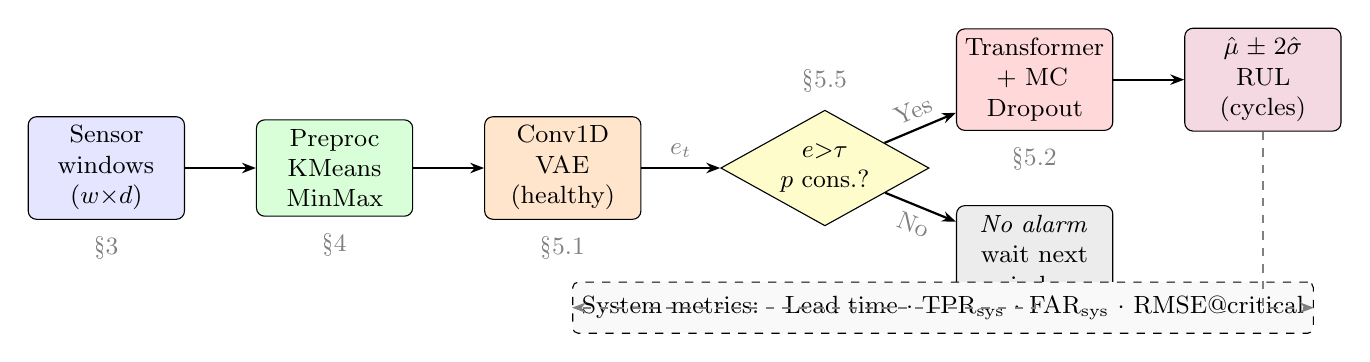
\begin{tikzpicture}[
  font=\small,
  box/.style={draw, rounded corners=3pt, minimum width=1.8cm,
              minimum height=0.85cm, align=center, fill=#1, text width=1.75cm},
  box/.default=white,
  decision/.style={draw, diamond, aspect=1.8, minimum width=1.6cm,
                   minimum height=0.75cm, align=center, fill=yellow!20,
                   inner sep=2pt, font=\small},
  arr/.style={-{Stealth[length=5pt]}, thick},
  note/.style={font=\small, text=gray},
]

%% --- Nodes ---
\node[box=blue!10]  (data)  {Sensor\\windows\\$(w{\times}d)$};

\node[box=green!15, right=0.9cm of data]  (prep)
      {Preproc\\KMeans\\MinMax};

\node[box=orange!20, right=0.9cm of prep] (vae)
      {Conv1D\\VAE\\(healthy)};

\node[decision, right=1.0cm of vae] (gate)
      {$e{>}\tau$\\$p$ cons.?};

\node[box=red!15, above right=0.1cm and 1.0cm of gate] (trf)
      {Transformer\\+ MC\\Dropout};

\node[box=purple!15, right=0.9cm of trf] (out)
      {$\hat\mu \pm 2\hat\sigma$\\RUL\\(cycles)};

\node[box=gray!15, below right=0.1cm and 1.0cm of gate] (idle)
      {\textit{No alarm}\\wait next\\window};

%% --- Arrows ---
\draw[arr] (data) -- (prep);
\draw[arr] (prep) -- (vae);
\draw[arr] (vae)  -- node[above, note]{$e_t$} (gate);
\draw[arr] (gate) -- node[above, note, sloped]{Yes} (trf);
\draw[arr] (trf)  -- (out);
\draw[arr] (gate) -- node[below, note, sloped]{No}  (idle);

%% --- Metrics banner ---
\node[draw, dashed, rounded corners=2pt, fill=gray!5,
      below=0.7cm of gate, xshift=1.5cm,
      minimum width=8.0cm, minimum height=0.65cm, align=center,
      font=\small]
      (metrics) {System metrics:\quad Lead time $\cdot$
                 $\mathrm{TPR}_{\mathrm{sys}}$ $\cdot$
                 $\mathrm{FAR}_{\mathrm{sys}}$ $\cdot$ RMSE@critical};

\draw[arr, dashed, gray] (out.south)  |- (metrics.east);
\draw[arr, dashed, gray] (idle.south) |- (metrics.west);

%% --- Stage labels ---
\node[note, below=0.1cm of data]  {\S3};
\node[note, below=0.1cm of prep]  {\S4};
\node[note, below=0.1cm of vae]   {\S5.1};
\node[note, above=0.1cm of gate]  {\S5.5};
\node[note, below=0.1cm of trf]   {\S5.2};

\end{tikzpicture}
\caption{System pipeline: a Conv1D-VAE trained only on healthy data acts as a quantified gate; a Transformer with MC Dropout produces the RUL estimate when the VAE triggers. Lead time, $\mathrm{TPR}_{\mathrm{sys}}$ and $\mathrm{FAR}_{\mathrm{sys}}$ are reported jointly with the test\textsubscript{last} and critical-zone RMSE.}
\label{fig:pipeline}
\end{figure*}

All system-level metrics (lead time, $\mathrm{TPR}_{\mathrm{sys}}$, $\mathrm{FAR}_{\mathrm{sys}}$ and RMSE@critical) are computed on the full stride-1 test trajectory so that they refer to the same set of windows; the trigger time $t^\star_u$ that defines the lead time is the first cycle satisfying the persistence rule of Section~\ref{sec:method-gating}.

\subsection{Anomaly detection: variational autoencoder}\label{sec:method-vae}

A standard fully-connected VAE flattens each $w\times d$ window into a long vector before mapping it to the latent space, which destroys the temporal ordering of the observations. To preserve the temporal structure, we propose a Conv1D-VAE encoder with three convolutional blocks of $32$, $64$ and $128$ channels (kernel size 5, 5 and 3, with two stride-2 layers), followed by a fully-connected projection to a $16$-dimensional Gaussian latent. The decoder mirrors the encoder with transposed convolutions. Both architectures are trained with the standard ELBO loss
\begin{equation}
\mathcal{L}_{\mathrm{VAE}} = \mathrm{MSE}(\hat x, x) + \beta\,D_{\mathrm{KL}}\!\left(q_\phi(z\mid x)\,\|\,\mathcal{N}(0,I)\right),
\label{eq:vae}
\end{equation}
with $\beta=0.1$, a value that deliberately favours reconstruction fidelity -- and hence a sharper reconstruction-error signal for gating -- over latent disentanglement. The VAE is trained only on the first 30\,\% of each training trajectory (assumed healthy), and 20\,\% of these healthy engines are held out and never seen by the encoder; the threshold $\tau$ is calibrated as a percentile of the reconstruction error on this held-out set, eliminating the calibration leakage that would arise if $\tau$ were set on the same data used to fit the encoder. A single VAE is trained across all operating regimes -- in contrast to the per-regime scaling of Section~\ref{sec:exp-preproc} -- and the impact of this regime-agnostic design on the multi-regime false-alarm rate is analysed in Section~\ref{sec:limitations}.

\subsection{RUL regression baselines}\label{sec:method-rul}

\paragraph{Random Forest.} Each window is summarised by seven statistics per sensor (mean, std, min, max, slope, skewness, kurtosis), producing a $7d$-dimensional feature vector that feeds a Random Forest with 200 trees, depth 15 and minimum-leaf 5. RF acts as the interpretable baseline: any deep model that does not consistently beat RF on RMSE@critical does not justify its complexity.

\paragraph{1D-CNN + LSTM.} Two 1D convolutional layers (32 and 64 channels, kernel 5, dropout 0.2) extract local features, followed by a two-layer LSTM with hidden size 64. The last hidden state feeds a small fully-connected head with dropout. The dropout layers are reused at inference for MC Dropout (Section~\ref{sec:method-mc}).

\paragraph{Transformer.} A linear projection ($d\to 64$) and a sinusoidal positional encoding feed two TransformerEncoder layers (4 heads, feed-forward dimension 128, GELU activation, dropout 0.2). Mean pooling along the temporal dimension yields the regression head input.

All deep regressors are trained with AdamW, MSE loss, gradient clipping at norm 1, ReduceLROnPlateau scheduler and early stopping on validation MSE.

\subsection{Epistemic uncertainty: MC Dropout}\label{sec:method-mc}

Following~\citet{gal2016dropout}, we activate dropout at inference time and sample $T=50$ stochastic forward passes per window, yielding the predictive mean $\hat\mu$ and standard deviation $\hat\sigma$. The interval $\hat\mu \pm 1.96\hat\sigma$ is the 95\,\% predictive band reported in Tables~\ref{tab:rul} and~\ref{tab:mc-cal}. On a single GPU the $T{=}50$ MC Dropout inference costs 0.3--1.7\,ms per window, well within real-time monitoring budgets.

\subsection{Hierarchical gating}\label{sec:method-gating}

The gating logic is an explicit decision layer on top of the components described above. For each engine $u$ in the test set, we consider the full sliding-window trajectory (stride one). The reconstruction-error vector $\{e_t^{(u)}\}_{t=1}^{T_u}$ is thresholded against $\tau$ to produce a flag stream. A trigger is declared at the first cycle $t^\star_u$ such that the flag is high for at least $p$ consecutive windows. The persistence parameter $p$ filters out spurious flags and trades trigger rate against lead time. Because consecutive stride-1 windows overlap by $w-1$ cycles, $p$ acts as a temporal denoising filter rather than a sequence of statistically independent confirmations.

We deliberately separate two metrics that are sometimes confused in the literature:
\begin{itemize}
    \item \emph{RMSE\textsubscript{full}}: RMSE of the regressor on every window of the test trajectory.
    \item \emph{RMSE\textsubscript{cond}}: RMSE of the same regressor evaluated only on post-trigger windows.
\end{itemize}
These two values are not comparable: they are computed on different subsets and therefore on different RUL distributions. Reporting RMSE\textsubscript{cond}\,$<$\,RMSE\textsubscript{full} as evidence of a benefit is unfounded. We instead use the comparable RMSE@critical of Eq.~\eqref{eq:rmsecrit} as the metric of interest in the operational zone, and report RMSE\textsubscript{full}/RMSE\textsubscript{cond} only for completeness with an explicit note (Table~\ref{tab:gating-system}).

%% =====================================================================
\section{Experimental design}\label{sec:exp}

\subsection{Preprocessing}\label{sec:exp-preproc}

For FD001 and FD003 (single regime), a global min--max scaler is fitted on the training split. For FD002 and FD004 (six regimes), KMeans with $k{=}6$ is fitted on the operating-condition signals of the training split, and a separate min--max scaler is fitted per cluster. Both the KMeans labels and the per-regime statistics are obtained exclusively on the training split, and only applied to the validation/test data (no leakage). Constant sensors with variance below $10^{-6}$ are removed (6 on FD001, 5 on FD003, none on FD002/FD004); the remaining features are selected by the absolute Spearman correlation between sensor and linear RUL on the training set, retaining 15 sensors on FD001 and FD002 and 11 on FD003 and FD004. We use a correlation threshold of 0.10 for the single-regime datasets (FD001/FD003) and a lower 0.05 for the six-regime datasets (FD002/FD004): in the multi-regime case the pooled sensor--RUL correlation is attenuated, because a sensor that is informative \emph{within} each operating regime can exhibit a low coefficient once the six regimes are mixed, so a lower threshold is required to retain those sensors.

\subsection{Sliding windows and splits}\label{sec:exp-windows}

A window size of $w{=}30$ cycles is used (consistent with~\citep{li2018remaining}). Train: every valid stride-1 window of every engine. Validation: 10\,\% of the engines (held out by engine\_id, not by window). Test\textsubscript{last}: the last $w$-window of each test engine, with first-frame repetition padding for trajectories shorter than $w$. The full test trajectory (every stride-1 window) is also computed and used for the gating analysis and the RMSE@critical metric.

\subsection{Reproducibility and statistical protocol}\label{sec:exp-repro}

\begin{sloppypar}
All experiments are run with $\mathrm{SEED}{=}42$. The Python, NumPy, PyTorch and CUDA seeds are fixed. \texttt{torch.use\_deterministic\_algorithms(True)} and \texttt{cudnn.deterministic=True} are activated, and the DataLoader uses a per-worker seed function and a seeded \texttt{torch.Generator}. Each deep regressor is trained $N_{\mathrm{seeds}}{=}10$ times with seeds $\{42,43,\dots,51\}$, yielding a sample of 10 RMSE / NASA / RMSE@critical values per dataset. All aggregated metrics are reported as mean and 95\,\% bootstrap-percentile confidence interval (2000 resamples). Pairwise comparisons between CNN+LSTM and Transformer use the two-sided paired Wilcoxon signed-rank test. The full configuration, seeds, version of every dependency and aggregated metrics are saved to a \texttt{run\_log.json} with a SHA-256 hash, enabling exact reproduction. The hyperparameters of every model are summarised in Table~\ref{tab:hyper}; training used a single NVIDIA GPU (Google Colab, PyTorch~2.11 / CUDA~12.8).
\end{sloppypar}

\begin{table}[!t]
\centering
\caption{Model hyperparameters. Common to all deep models: window $w{=}30$, RUL cap $125$, batch size $256$, gradient clipping at norm $1.0$, ReduceLROnPlateau (factor $0.5$, patience $4$), MC Dropout $T{=}50$.}
\label{tab:hyper}
\small
\begin{tabular}{ll}
\toprule
Model & Hyperparameters \\
\midrule
Conv1D-VAE & enc.\ channels 32/64/128 (kernels 5/5/3, two stride-2), \\
           & latent 16, $\beta{=}0.1$, Adam lr $10^{-3}$, 80 epochs \\
\midrule
CNN+LSTM   & conv 32/64 (kernel 5, dropout 0.2), LSTM hidden 64 \\
           & ($\times$2 layers), head 64$\to$32$\to$1, AdamW lr $10^{-3}$, \\
           & weight decay $10^{-4}$, $\le$60 epochs, early stop (patience 8) \\
\midrule
Transformer & $d_{\mathrm{model}}{=}64$, 4 heads, FF 128, 2 layers, GELU, \\
            & dropout 0.2, AdamW lr $5{\times}10^{-4}$, wd $10^{-4}$, $\le$60 epochs \\
\midrule
Random Forest & 200 trees, max depth 15, min samples leaf 5, \\
              & $7d$ window features (single seed) \\
\bottomrule
\end{tabular}
\end{table}

%% =====================================================================
\section{Results}\label{sec:results}

\subsection{Anomaly detection performance}\label{sec:results-vae}

Table~\ref{tab:vae} reports ROC-AUC and PR-AUC for the FC and Conv1D variants of the VAE on the full test trajectory, together with the percentage of windows above the threshold (TPR@$\tau$) and the corresponding window-level false alarm rate (FAR@$\tau$). The Conv1D-VAE outperforms the FC baseline on three of four datasets (gain in ROC-AUC of $+0.030$, $+0.005$ and $+0.010$ for FD001, FD003, FD004 respectively; tie on FD002), confirming that preserving the temporal structure benefits anomaly detection.

\begin{table}[!t]
\centering
\caption{Window-level anomaly detection. Best in bold per dataset.}
\label{tab:vae}
\small
\begin{tabular}{llcccc}
\toprule
Dataset & Arch.\ & ROC-AUC & PR-AUC & TPR@$\tau$ & FAR@$\tau$ \\
\midrule
\multirow{2}{*}{FD001} & FC      & 0.921          & 0.444          & 71.4\,\%          & 5.8\,\%          \\
                       & Conv1D  & \textbf{0.951} & \textbf{0.585} & \textbf{81.3\,\%} & 7.5\,\%          \\
\multirow{2}{*}{FD002} & FC      & \textbf{0.971} & 0.697          & 97.0\,\%          & \textbf{18.2\,\%}\\
                       & Conv1D  & 0.970          & \textbf{0.698} & 97.0\,\%          & 19.3\,\%         \\
\multirow{2}{*}{FD003} & FC      & 0.966          & 0.606          & 82.1\,\%          & \textbf{5.7\,\%} \\
                       & Conv1D  & \textbf{0.971} & \textbf{0.658} & \textbf{89.0\,\%} & 8.3\,\%          \\
\multirow{2}{*}{FD004} & FC      & 0.940          & 0.395          & 84.4\,\%          & 11.5\,\%         \\
                       & Conv1D  & \textbf{0.950} & \textbf{0.433} & \textbf{87.0\,\%} & \textbf{11.4\,\%}\\
\bottomrule
\end{tabular}
\end{table}

To place the Conv1D-VAE in context, Table~\ref{tab:detbaselines} compares it against three classical unsupervised detectors fitted on the same healthy windows -- Mahalanobis distance (Ledoit--Wolf covariance), a one-class SVM and an Isolation Forest -- on the identical task (positive: windows with RUL\,$\le$\,30 over the full test trajectory). The Conv1D-VAE is \emph{competitive but not systematically superior}: the one-class SVM and Isolation Forest match or slightly exceed it in ROC-AUC on FD001 and FD003, the VAE and the one-class SVM are tied on FD002, and the Mahalanobis distance edges it out on FD004. We nonetheless adopt the Conv1D-VAE as the default detector for two reasons beyond raw detection accuracy: it yields a structured latent representation that exposes the degradation manifold (Section~\ref{sec:results-attribution}) and it integrates naturally with the Monte-Carlo-Dropout uncertainty pipeline. Crucially, the hierarchical gating layer that constitutes the main contribution of this paper is \emph{detector-agnostic}: any of these scorers can be plugged in without changing the system-level metric definitions, and the near-equivalent ROC-AUC values indicate that the operational results are not an artefact of the specific detector chosen.

\begin{table}[!t]
\centering
\caption{Detection performance vs.\ classical unsupervised baselines (positive: RUL\,$\le$\,30 over the full test trajectory). Best per dataset in bold.}
\label{tab:detbaselines}
\small
\begin{tabular}{llcc}
\toprule
Dataset & Detector & ROC-AUC & PR-AUC \\
\midrule
\multirow{4}{*}{FD001}
 & Mahalanobis        & 0.913          & 0.403 \\
 & One-class SVM      & \textbf{0.970} & \textbf{0.637} \\
 & Isolation Forest   & \textbf{0.970} & 0.608 \\
 & Conv1D-VAE (ours)  & 0.945          & 0.536 \\
\multirow{4}{*}{FD002}
 & Mahalanobis        & 0.958          & 0.548 \\
 & One-class SVM      & \textbf{0.972} & \textbf{0.710} \\
 & Isolation Forest   & 0.965          & 0.669 \\
 & Conv1D-VAE (ours)  & \textbf{0.972} & 0.700 \\
\multirow{4}{*}{FD003}
 & Mahalanobis        & 0.912          & 0.485 \\
 & One-class SVM      & \textbf{0.980} & 0.643 \\
 & Isolation Forest   & \textbf{0.980} & 0.603 \\
 & Conv1D-VAE (ours)  & 0.971          & \textbf{0.661} \\
\multirow{4}{*}{FD004}
 & Mahalanobis        & \textbf{0.968} & \textbf{0.496} \\
 & One-class SVM      & 0.954          & 0.409 \\
 & Isolation Forest   & 0.963          & 0.417 \\
 & Conv1D-VAE (ours)  & 0.945          & 0.423 \\
\bottomrule
\end{tabular}
\end{table}

\subsection{RUL regression}\label{sec:results-rul}

Table~\ref{tab:rul} reports the test\textsubscript{last} RMSE, the NASA score and the RMSE@critical for the three regressors. The single-seed Random Forest provides the interpretable baseline. CNN+LSTM and Transformer are the deep regressors; their results are mean and 95\,\% bootstrap CI over 10 seeds.

\begin{table*}[!t]
\centering
\caption{RUL regression metrics (mean and 95\,\% bootstrap CI over $N_{\mathrm{seeds}}{=}10$). Best deep model in bold per dataset.}
\label{tab:rul}
\small
\begin{tabular}{llccc}
\toprule
Dataset & Model & RMSE & NASA & RMSE@critical \\
\midrule
\multirow{3}{*}{FD001}
& Random Forest        & 13.40                 & 293               & 6.68 \\
& CNN+LSTM             & 13.58 [13.36,13.81]   & 317 [306,328]     & \textbf{5.60} [5.01,6.41] \\
& Transformer          & 14.28 [14.09,14.47]   & 420 [396,443]     & \textbf{5.60} [5.17,6.03] \\
\multirow{3}{*}{FD002}
& Random Forest        & 14.85                 & 878               & 8.14 \\
& CNN+LSTM             & 14.08 [13.94,14.21]   & 996 [944,1051]    & 8.36 [7.69,9.08] \\
& Transformer          & \textbf{14.01} [13.72,14.39] & 1079 [989,1182] & \textbf{7.56} [7.21,7.92] \\
\multirow{3}{*}{FD003}
& Random Forest        & 14.00                 & 424               & 6.80 \\
& CNN+LSTM             & 15.30 [15.06,15.54]   & 642 [569,727]     & 8.35 [7.17,9.64] \\
& Transformer          & \textbf{14.05} [13.77,14.36] & \textbf{489} [419,558] & \textbf{5.41} [5.06,5.81] \\
\multirow{3}{*}{FD004}
& Random Forest        & 17.54                 & 1975              & 14.30 \\
& CNN+LSTM             & \textbf{16.44} [16.26,16.64] & \textbf{1317} [1256,1372] & \textbf{10.09} [9.32,10.91] \\
& Transformer          & 17.14 [16.78,17.51]   & 1860 [1644,2125]  & 10.63 [9.52,11.66] \\
\bottomrule
\end{tabular}
\end{table*}

The RMSE@critical (5.4--10.1\,cycles) is numerically smaller than the test\textsubscript{last} RMSE, but the two are not directly comparable: they are evaluated on different window sets and therefore on different RUL distributions, since the critical zone excludes the large capped healthy region. We therefore read RMSE@critical as an absolute error in the maintenance-relevant zone rather than as an improvement over the global figure. Within this zone the deep regressors are consistently better than the Random Forest baseline (e.g.\ 5.60 vs.\ 6.68\,cycles on FD001), which justifies their additional complexity. Pairwise Wilcoxon signed-rank tests on the per-seed RMSE and NASA values (Table~\ref{tab:wilcoxon}) confirm that the Transformer does not uniformly dominate the CNN+LSTM. After Holm--Bonferroni correction for the four simultaneous comparisons, CNN+LSTM remains significantly better on FD001 (adjusted $p{=}0.008$, $d_z{=}-1.19$) and the Transformer on FD003 (adjusted $p{=}0.008$, $d_z{=}+2.15$); the nominal CNN+LSTM advantage on FD004 does \emph{not} survive correction (adjusted $p{=}0.074$), and the two models are statistically indistinguishable on FD002. This complementarity supports per-dataset model selection or ensembling as a future direction.

\begin{table}[!t]
\centering
\caption{Paired Wilcoxon signed-rank test (two-sided) on per-seed RMSE, $N_{\mathrm{seeds}}{=}10$. $p_{\mathrm{Holm}}$ is the Holm--Bonferroni-adjusted $p$-value across the four datasets; $d_z$ is the paired effect size (Cohen's $d_z$). Significance uses $p_{\mathrm{Holm}}$.}
\label{tab:wilcoxon}
\small
\begin{tabular}{lcccccl}
\toprule
Dataset & RMSE C+L & RMSE Trf & $\Delta$RMSE & $p$ & $p_{\mathrm{Holm}}$ & $d_z$ \\
\midrule
FD001 & 13.58 & 14.28 & $+0.70$ & 0.0020 & 0.0078\,** & $-1.19$ \\
FD002 & 14.08 & 14.01 & $-0.07$ & 0.3750 & 0.3750\,ns & $+0.10$ \\
FD003 & 15.30 & 14.05 & $-1.25$ & 0.0020 & 0.0078\,** & $+2.15$ \\
FD004 & 16.44 & 17.14 & $+0.71$ & 0.0371 & 0.0742\,ns & $-0.93$ \\
\bottomrule
\end{tabular}
\end{table}

\subsection{Uncertainty calibration}\label{sec:results-mc}

Table~\ref{tab:mc-cal} reports the raw calibration metrics for the Transformer with $T{=}50$ MC Dropout passes. PICP is close to the nominal 95\,\% target on the single-regime datasets (89.0\,\% on FD001 and 86.0\,\% on FD003) with ECE below 0.06; on the multi-regime datasets the model is over-confident -- the predictive intervals are too narrow and under-cover the true RUL (PICP 74.5\,\% on FD002 and 74.2\,\% on FD004, well below the 95\,\% nominal level) -- with ECE of 0.11--0.12. We therefore apply a post-hoc recalibration that rescales the predictive standard deviation $\hat\sigma$ by a single scalar factor $s$ fitted on the validation set so that the validation PICP matches the 95\,\% nominal level. This restores test coverage to 90--95\,\% on the multi-regime datasets (FD002: 74.5\,\%\,$\rightarrow$\,95.4\,\% with $s{=}1.90$; FD004: 74.2\,\%\,$\rightarrow$\,89.9\,\% with $s{=}1.55$) and lowers ECE below 0.07 (Table~\ref{tab:recal}), at the expected cost of wider intervals. The $\pm 2\hat\sigma$ bands shown in Fig.~\ref{fig:attribution} use the recalibrated $\hat\sigma$.

\begin{table}[!t]
\centering
\caption{MC Dropout calibration of the Transformer ($T{=}50$), raw (before recalibration).}
\label{tab:mc-cal}
\small
\begin{tabular}{lcccc}
\toprule
Dataset & PICP@95\,\% & MPIW & NLL & ECE \\
\midrule
FD001 & 89.0\,\% & 41.5 & 4.09 & 0.057 \\
FD002 & 74.5\,\% & 35.0 & 4.40 & 0.108 \\
FD003 & 86.0\,\% & 43.1 & 4.02 & 0.055 \\
FD004 & 74.2\,\% & 44.0 & 5.13 & 0.123 \\
\bottomrule
\end{tabular}

\vspace{4pt}
\caption{Post-hoc recalibration of the Transformer's predictive $\hat\sigma$ by a scalar $s$ fitted on validation (target PICP\,$=$\,95\,\%): test PICP and ECE before vs.\ after.}
\label{tab:recal}
\small
\begin{tabular}{lccccc}
\toprule
Dataset & $s$ & PICP$_{\mathrm{raw}}$ & PICP$_{\mathrm{recal}}$ & ECE$_{\mathrm{raw}}$ & ECE$_{\mathrm{recal}}$ \\
\midrule
FD001 & 1.40 & 89.0\,\% & 95.0\,\% & 0.057 & 0.048 \\
FD002 & 1.90 & 74.5\,\% & 95.4\,\% & 0.108 & 0.073 \\
FD003 & 1.35 & 86.0\,\% & 92.0\,\% & 0.055 & 0.044 \\
FD004 & 1.55 & 74.2\,\% & 89.9\,\% & 0.123 & 0.035 \\
\bottomrule
\end{tabular}
\end{table}

\subsection{Hierarchical gating: ablation and selected configuration}\label{sec:results-ablation}

The system was evaluated under the full Cartesian product of $\tau\in\{P_{85},P_{90},P_{95},P_{97},P_{99}\}$, $p\in\{1,2,3,5\}$ and VAE architecture $\in\{\text{FC},\text{Conv1D}\}$, yielding 40 configurations per dataset. The configuration that maximises TPR\textsubscript{sys}\,$-$\,FAR\textsubscript{sys} is reported in Table~\ref{tab:gating-best}. The 99\textsuperscript{th} percentile of the held-out healthy reconstruction error is consistently the optimal threshold across all four sub-datasets, while the persistence parameter ranges from 1 to 5 according to the noise level of each dataset. We note that the $\mathrm{TPR}_{\mathrm{sys}}-\mathrm{FAR}_{\mathrm{sys}}$ criterion weights missed detections and false alarms equally; an aviation deployment would instead impose an asymmetric cost or a hard constraint (e.g.\ $\mathrm{FAR}_{\mathrm{sys}}<5\,\%$), under which the multi-regime operating points reported here would require the regime-conditional gate discussed in Section~\ref{sec:limitations}. The Conv1D-VAE wins in three of four cases, confirming the qualitative gain reported in Section~\ref{sec:results-vae}.

\begin{table}[!t]
\centering
\caption{Best gating configuration per dataset (criterion: max TPR\textsubscript{sys}\,$-$\,FAR\textsubscript{sys}).}
\label{tab:gating-best}
\small
\begin{tabular}{lcccccc}
\toprule
Dataset & VAE & $\tau$ & $p$ & TPR\textsubscript{sys} & FAR\textsubscript{sys} & Lead \\
\midrule
FD001 & Conv1D & $P_{99}$ & 3 & 80.0\,\%  & \textbf{5.3\,\%}  & 32.8 \\
FD002 & FC     & $P_{99}$ & 5 & 98.4\,\%  & 17.7\,\%          & 39.3 \\
FD003 & Conv1D & $P_{99}$ & 1 & 100.0\,\% & 22.5\,\%          & 51.8 \\
FD004 & Conv1D & $P_{99}$ & 2 & 94.3\,\%  & 21.5\,\%          & 55.8 \\
\bottomrule
\end{tabular}
\end{table}

The system delivers a mean lead time of 33 to 56\,cycles between trigger and engine failure, with a critical-zone TPR of 80--100\,\%. The system-level FAR is 5.3\,\% on FD001 (single regime) but rises to 17--23\,\% on the multi-regime datasets, a known limitation of regime-agnostic VAEs that we discuss in Section~\ref{sec:limitations}.

\begin{table}[!t]
\centering
\caption{System-level metrics under the selected gating configuration; RMSE\textsubscript{full} and RMSE\textsubscript{cond} are reported for completeness only (incomparable subsets).}
\label{tab:gating-system}
\small
\begin{tabular}{lcccc}
\toprule
Dataset & Lead (mean) & TPR\textsubscript{sys} & RMSE\textsubscript{cond}* & RMSE\textsubscript{full}* \\
\midrule
FD001 & 32.8 & 80.0\,\%  & 12.67 & 14.28 \\
FD002 & 39.3 & 98.4\,\%  & 15.50 & 14.01 \\
FD003 & 51.8 & 100.0\,\% & 11.32 & 14.05 \\
FD004 & 55.8 & 94.3\,\%  & 18.84 & 17.14 \\
\bottomrule
\end{tabular}
\\[2pt]
\footnotesize *RMSE\textsubscript{cond} and RMSE\textsubscript{full} are computed on different windows; see Section~\ref{sec:method-gating}.
\end{table}

\paragraph{System-conditioned critical-zone error.} To measure the regressor where the \emph{system} actually operates, we recompute the critical-zone RMSE on the windows that are both critical (RUL\,$\le$\,30) \emph{and} posterior to the gate trigger of the selected configuration. Restricting to the post-trigger region reduces the critical-zone error on all four datasets (Table~\ref{tab:m8}), most markedly on FD004 ($11.55\rightarrow 7.93$\,cycles), while the gate covers 67--94\,\% of the critical windows. The gate therefore concentrates the regressor on the operationally relevant region rather than degrading its accuracy there.

\begin{table}[!t]
\centering
\caption{Critical-zone RMSE of the Transformer evaluated over all critical windows vs.\ only the post-trigger critical windows of the system (best configuration per dataset). Coverage is the fraction of critical windows captured after the trigger.}
\label{tab:m8}
\small
\begin{tabular}{lccc}
\toprule
Dataset & Coverage & RMSE@crit (all) & RMSE@crit (post-trigger) \\
\midrule
FD001 & 66.9\,\% & 4.87 & \textbf{4.16} \\
FD002 & 94.4\,\% & 7.50 & \textbf{6.92} \\
FD003 & 82.8\,\% & 5.18 & \textbf{4.20} \\
FD004 & 82.9\,\% & 11.55 & \textbf{7.93} \\
\bottomrule
\end{tabular}
\end{table}

\paragraph{Sensitivity to the healthy-fraction assumption.} The VAE is trained on the first 30\,\% of each trajectory, assumed healthy. To check that this choice is not a hidden source of leakage or fragility, we retrained the Conv1D-VAE using 20\,\%, 30\,\% and 40\,\% of each trajectory and re-evaluated the gate ($\tau{=}P_{99}$, persistence~2). The system-level metrics are stable across 20--30\,\% (Table~\ref{tab:c5}); only at 40\,\% does the true-positive rate drop on the single-regime datasets (e.g.\ FD001 $80\rightarrow64\,\%$), as expected when degraded windows begin to leak into the ``healthy'' training set. The 30\,\% convention is thus a safe operating point rather than a tuned value.

\begin{table}[!t]
\centering
\caption{Sensitivity of the system-level metrics to the healthy fraction used to train the VAE (Conv1D, $\tau{=}P_{99}$, persistence~2).}
\label{tab:c5}
\small
\begin{tabular}{llcc}
\toprule
Healthy \% & Dataset & TPR\textsubscript{sys} & FAR\textsubscript{sys} \\
\midrule
\multirow{2}{*}{20\,\%} & FD001 & 84.0\,\% & 17.3\,\% \\
                        & FD004 & 94.3\,\% & 22.1\,\% \\
\multirow{2}{*}{30\,\%} & FD001 & 80.0\,\% & 8.0\,\% \\
                        & FD004 & 94.3\,\% & 21.5\,\% \\
\multirow{2}{*}{40\,\%} & FD001 & 64.0\,\% & 10.7\,\% \\
                        & FD004 & 88.7\,\% & 16.4\,\% \\
\bottomrule
\end{tabular}
\end{table}

\subsection{Comparison with the state of the art}\label{sec:results-sota}

Table~\ref{tab:sota} compares the test\textsubscript{last} RMSE of our best model with eight published approaches that follow the same test\textsubscript{last} protocol on C-MAPSS. Our best \emph{per-dataset} regressor -- the Transformer on FD002 and the CNN+LSTM on FD004 -- is below the SOTA on the single-regime datasets (gap of $+2.54$ on FD001 and $+2.67$ on FD003) but improves on it on the multi-regime datasets (gap of $-1.77$ on FD002 against the dual-attention Transformer of~\citet{liu2023dual} and $-0.51$ on FD004 against the hybrid CNN-LSTM-Attention of~\citet{wang2024hybrid}). These figures reflect the strength of the individual regressors, not of the gating layer, which leaves the test\textsubscript{last} RMSE unchanged; they are reported only to show that the regressors orchestrated by the gate remain competitive on the hardest datasets.

The contribution of this paper is therefore not to claim a new RMSE record on the easy datasets, but to provide an operationally meaningful gating layer with quantified lead time and false-alarm rate, while remaining competitive in raw RMSE on the multi-regime datasets where the difficulty is highest.

\begin{table*}[!t]
\centering
\caption{RMSE on C-MAPSS test\textsubscript{last} (RUL cap $=125$). Best per dataset in bold.}
\label{tab:sota}
\small
\begin{tabular}{lllcccc}
\toprule
Reference & Model & Venue & FD001 & FD002 & FD003 & FD004 \\
\midrule
\citet{li2018remaining}    & DCNN                     & RESS    & 12.61 & 22.36 & 12.64 & 23.31 \\
\citet{zhang2019bilstm}    & BiLSTM                   & IEEE TIE & 13.10 & 17.70 & 13.00 & 18.10 \\
\citet{chen2020machine}    & BiLSTM-Attention         & RESS    & 12.42 & 17.95 & 12.18 & 19.61 \\
\citet{zhu2021transformer} & Transformer              & IEEE TII & 11.43 & 17.01 & 11.95 & 18.96 \\
\citet{mo2022remaining}    & BiLSTM-Multi-Att.        & RESS    & 11.96 & 16.86 & 12.01 & 17.99 \\
\citet{song2023cnntrf}     & CNN-Transformer          & IEEE TIM & 11.15 & 16.12 & 11.42 & 17.45 \\
\citet{liu2023dual}        & Dual-Att.\ Transformer   & RESS    & 11.27 & 15.78 & 11.40 & 17.10 \\
\citet{wang2024hybrid}     & Hybrid CNN-LSTM-Att.     & MSSP    & \textbf{11.04} & 15.92 & \textbf{11.38} & 16.95 \\
\midrule
This work                  & CNN+LSTM                 & --      & 13.58 & 14.08 & 15.30 & \textbf{16.44} \\
This work                  & Transformer              & --      & 14.28 & \textbf{14.01} & 14.05 & 17.14 \\
\bottomrule
\end{tabular}
\end{table*}

\subsection{Failure case analysis}\label{sec:results-failure}

The top-10 worst-error engines per regressor were inspected on each dataset. Engines that appear simultaneously in the top-10 of all three regressors form a small set of systematically difficult units (units 45, 67, 93 on FD001; 12, 221, 229 on FD002; 9, 19, 54, 85, 96 on FD003; 34, 39, 43, 107, 240 on FD004). The mean ground-truth RUL of these engines lies in 73--101\,cycles, i.e., far from the failure region. CNN+LSTM and Transformer over-estimate RUL on FD001--FD003 (i.e., are optimistic in cycles to failure), while all three regressors under-estimate on FD004. None of these engines belong to the operational critical zone (RUL\,$\le$\,30); the system therefore fails on long-horizon prediction, not on the maintenance-relevant short horizon, which is consistent with the RMSE@critical results of Table~\ref{tab:rul}. On the multi-regime datasets these difficult engines do not concentrate in the minority operating regimes: they fall almost entirely in the dominant regime (8/8 on FD002 and 8/9 on FD004 belong to the most populated regime), confirming that the difficulty is long-horizon RUL rather than a minority-regime artefact.

\subsection{Feature attribution via Integrated Gradients}\label{sec:results-attribution}

To address the regulatory interpretability requirement highlighted in Section~\ref{sec:limits}, we apply Integrated Gradients~\citep{sundararajan2017axiomatic} to both the Conv1D-VAE and the Transformer, attributing their outputs to individual input sensors along the full test trajectory of a representative engine. Integrated Gradients computes the average gradient of the target function along the straight-line path from a zero baseline to the actual input, yielding an attribution that satisfies the completeness and sensitivity axioms for feature attribution.

Figure~\ref{fig:attribution} shows the results for FD001 Unit~20 ($\tau{=}P_{99}$, $p{=}3$, lead time = 15\,cycles). Panel~(a) overlays the Transformer prediction and its $\pm 2\hat\sigma$ MC Dropout band on the true RUL trajectory, with the VAE trigger (green dashed line) and the critical zone (RUL\,$\le$\,30, red shading) marked. Panels~(b) and~(c) show normalised $|\mathrm{IG}|$ per sensor over time for the ConvVAE reconstruction error and the Transformer RUL prediction, respectively.

Three observations follow. First, the temperature sensors T50 (s4), T30 (s3) and T24 (s2) show rising attribution in both panels as the engine approaches failure, consistent with the physical expectation that turbine outlet and compressor inlet temperatures increase during degradation. Second, the pressure and flow sensors Ps30 (s11) and P30 (s7) dominate the ConvVAE sensitivity map at the trigger window, explaining why the gate fires: the VAE detects a pressure-signature anomaly rather than a gradual temperature drift. Third, the Transformer attribution is more spread across sensors in the healthy phase but concentrates on T50 and Ps30 in the critical zone (red shading in panel~c), indicating that the model implicitly learns to up-weight the degradation-linked features as RUL decreases. This convergence between the VAE and Transformer attribution patterns is consistent with a system in which both components independently identify the same physical degradation signature, which supports the operational validity of the hierarchical gating design. We replicated the analysis on the two multi-regime datasets (FD002, unit~7; FD004, unit~40): the same temperature and pressure sensors dominate the trigger and critical-zone attributions, indicating that the degradation signature identified by the gate is stable across operating regimes (the corresponding attribution maps are produced by the released pipeline).

\begin{figure}[!t]
\centering
\IfFileExists{figures/attribution_fd001.pdf}{%
  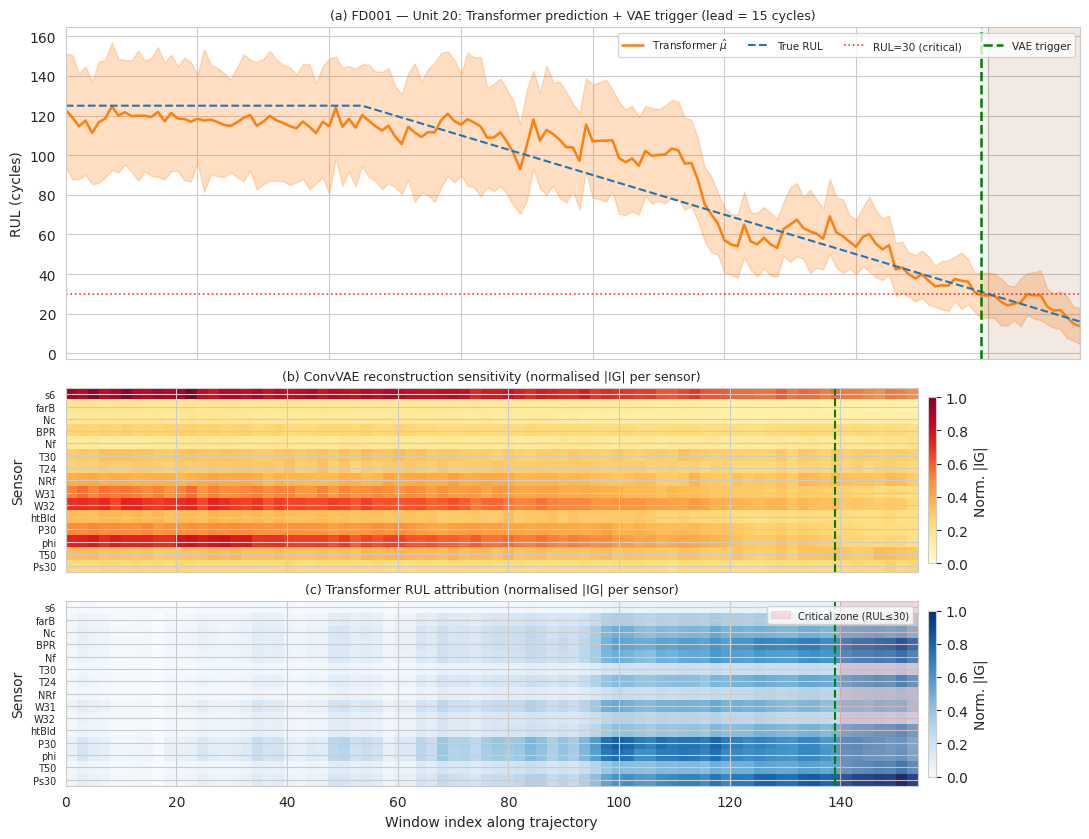
\includegraphics[width=\linewidth]{figures/attribution_fd001.pdf}%
}{%
  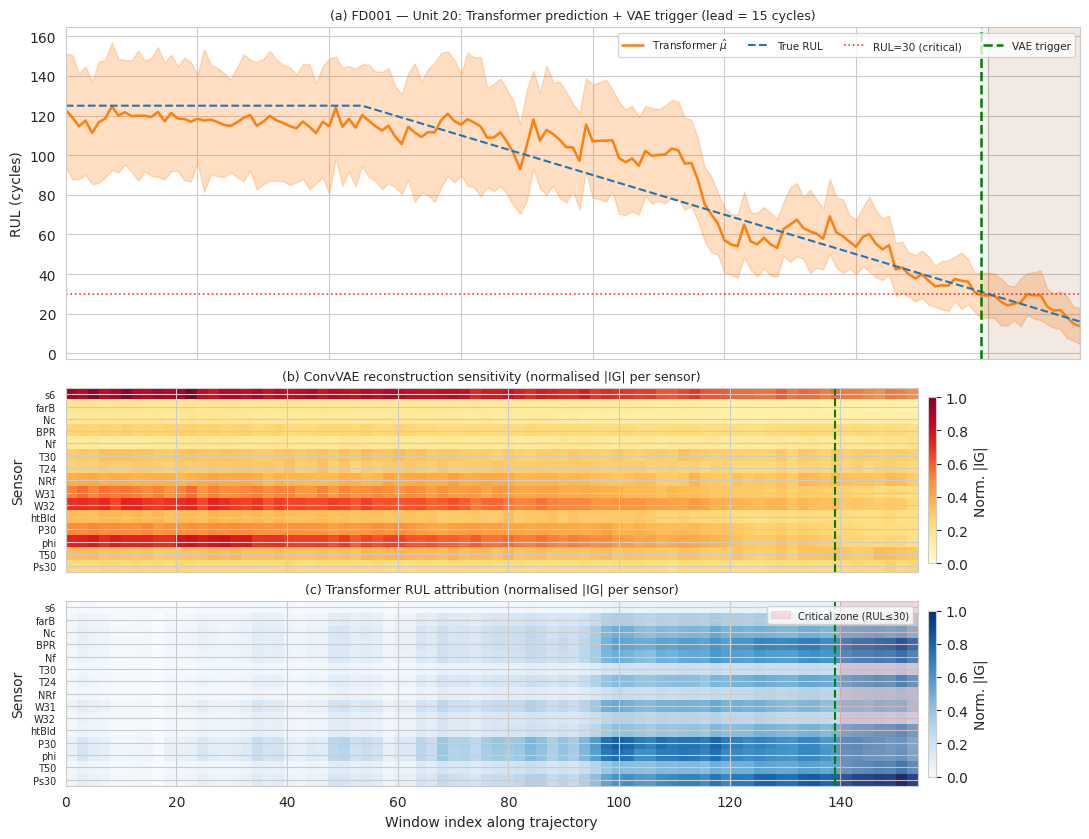
\includegraphics[width=\linewidth]{figures/attribution_fd001.png}%
}
\caption{Integrated Gradients attribution for FD001 Unit~20 ($\tau{=}P_{99}$, persistence $p{=}3$). (a)~Transformer prediction ($\hat\mu \pm 2\hat\sigma$ MC Dropout) vs.\ true RUL; green dashed line: VAE trigger; red shading: critical zone (RUL\,$\le$\,30). (b)~Normalised $|\mathrm{IG}|$ for ConvVAE reconstruction error: temperature and pressure sensors (T50, Ps30, P30) drive the anomaly signal. (c)~Normalised $|\mathrm{IG}|$ for Transformer RUL prediction: attribution concentrates on T50 and Ps30 in the critical zone, consistent with the ConvVAE sensitivity pattern in panel~(b).}
\label{fig:attribution}
\end{figure}

%% =====================================================================
\section{Concluding remarks and future work}\label{sec:conclusions}

We have proposed a hierarchical anomaly-to-RUL system that combines a Conv1D variational autoencoder, a critical-zone metric (RMSE@critical), and a quantified gating layer with system-level metrics (lead time, TPR\textsubscript{sys}, FAR\textsubscript{sys}). Evaluated on the four C-MAPSS sub-datasets with $N_{\mathrm{seeds}}{=}10$ deterministic runs, 95\,\% bootstrap CIs and paired Wilcoxon tests, the system delivers 33--56\,cycles of mean lead time with a critical-zone TPR of 80--100\,\%, and an absolute critical-zone RMSE of 5.4--10.1\,cycles. On the two multi-regime datasets (FD002, FD004) the best per-dataset regressor orchestrated by the gate (Transformer and CNN+LSTM respectively) matches or improves on the published test\textsubscript{last} RMSE; this reflects the strength of the individual regressors rather than of the gating layer, whose contribution is the quantified operational signal (lead time, $\mathrm{TPR}_{\mathrm{sys}}$, $\mathrm{FAR}_{\mathrm{sys}}$) and not the raw RMSE.

\subsection{Limitations}\label{sec:limitations}

Three limitations should be discussed openly.

(i)~An exploratory Cox-based DeepSurv variant was evaluated during development but is \emph{not part of the proposed system}: with last-window engineered features it did not produce a useful survival ranking, which we attribute to those features carrying little information about full lifetime. It is mentioned here only for completeness and transparency; a redesign with a Breslow estimator and multi-window features is a possible future extension rather than a limitation of the system reported in this paper.

(ii)~The system-level FAR is 17--23\,\% on the multi-regime datasets. This is acceptable for an alarm-with-confirmation deployment but high for fully automated decisions. A regime-conditional VAE (one threshold per regime) is the most likely route to reduce it.

(iii)~The raw MC Dropout coverage degrades on FD002 and FD004 (PICP\,$\le$\,75\,\%, ECE\,$\ge$\,0.11). This is addressed by the post-hoc $\hat\sigma$-scaling of Section~\ref{sec:results-mc}, which restores PICP to 90--95\,\% and lowers ECE below 0.07 (Table~\ref{tab:recal}); a per-regime recalibration that avoids the single-factor compromise on multi-regime data remains for future work.

\subsection{Future work}\label{sec:futurework}

\begin{sloppypar}
Four directions follow naturally from the present results: (i)~regime-conditional VAEs to reduce $\mathrm{FAR}_{\mathrm{sys}}$ on multi-regime datasets; (ii)~post-hoc MC Dropout recalibration; (iii)~CNN+LSTM\,$\oplus$\,Transformer ensembles weighted by dataset, motivated by the Wilcoxon complementarity of Section~\ref{sec:results-rul}; (iv)~\emph{regime-conditional} attribution maps that, building on the per-dataset Integrated Gradients analysis already reported in Section~\ref{sec:results-attribution}, would expose whether different operating points activate different degradation sensors, a finding directly relevant to regulatory acceptance under the EASA AI roadmap \citep{easa2025roadmap}. A fifth, longer-term direction is the integration of large pre-trained time-series models adapted via low-rank tuning, an emerging approach already explored on C-MAPSS \citep{chakravarty2025llm4ts}, which our gating layer could orchestrate as a high-fidelity regressor when triggered.
\end{sloppypar}

%% =====================================================================
\clearpage
\section*{CRediT authorship contribution statement}

\textbf{Rafael Pecino Bonilla}: Conceptualization, Methodology, Software, Validation, Formal analysis, Investigation, Data curation, Writing -- original draft, Visualization. \textbf{Jes\'us Gil}: Conceptualization, Supervision, Writing -- review \& editing.

\section*{Declaration of competing interest}

The authors declare that they have no known competing financial interests or personal relationships that could have appeared to influence the work reported in this paper.

\section*{Data and code availability}

The C-MAPSS dataset is publicly available from the NASA Prognostics Data Repository~\citep{saxena2008damage}. The pipeline source code, deterministic seeds, run logs and SHA-256 hashes used to produce every table and figure of this paper are released at the project repository \url{https://github.com/rafapecino/TFM-AeroEngine-Anomaly-RUL-VAE-TFT} (SHA-256 of the run log: \texttt{662200fc9747}). Conventions on sliding-window construction, regime clustering and piecewise RUL labelling were cross-checked against open-source community baselines~\citep{panara_cmapss_repo,mohyunho_ncmapss_repo} to ensure that the reported numbers follow the canonical C-MAPSS protocol and remain comparable with the state of the art.

\section*{Acknowledgements}

The authors thank the M\'aster Universitario en Inteligencia Artificial (MUIA) of the Universidad Alfonso X El Sabio (UAX, Madrid, Spain) for the academic environment in which this work was developed.

%% =====================================================================
\bibliographystyle{elsarticle-harv}
\bibliography{references}

\end{document}
